Primero creamos el proyecto al cual le agregaremos la funcionalidad de excel.


\begin{lstlisting}[language=bash]
$ flutter create leer_excel
\end{lstlisting}

 Posteriormente debemos agregar el paquete de Excel a su archivo \textbf{pubspec.yaml}. Haga clic en el "excel" de arriba para obtener la última versión del paquete de Excel. Actualmente estoy usando:

\begin{lstlisting}[language=bash]
dependencies:
	excel: ^1.1.5
\end{lstlisting}

Ahora necesitamos agregar la importación de la librería, para ello creamos el archivo \textbf{\textit{leer\_excel.dart}} en donde escribiremos el programa de importación de excel.

\begin{lstlisting}[language=c]
import  'package:excel/excel.dart';
\end{lstlisting}

Se modifica el programa principal

\begin{lstlisting}[language=c]
import 'package:flutter/material.dart';
import 'package:leer_excel/leer_excel.dart';

void main() {
	runApp(const MiApp());
}

class MiApp extends StatelessWidget {
	const MiApp({Key? key}) : super(key: key);
	
	// This widget is the root of your application.
	@override
	Widget build(BuildContext context) {
		return MaterialApp(
		title: 'Lectura de Excel',
		theme: ThemeData(
		// This is the theme of your application.
		//
		// Try running your application with "flutter run". You'll see the
		// application has a blue toolbar. Then, without quitting the app, try
		// changing the primarySwatch below to Colors.green and then invoke
		// "hot reload" (press "r" in the console where you ran "flutter run",
		// or simply save your changes to "hot reload" in a Flutter IDE).
		// Notice that the counter didn't reset back to zero; the application
		// is not restarted.
		primarySwatch: Colors.blue,
		),
		home: LeerExcel(),
		);
	}
}
\end{lstlisting}

El archivo de leer\_excel.dart queda de la siguiente forma:

\begin{lstlisting}[language=java]
import 'package:excel/excel.dart';
import 'package:flutter/material.dart';
import 'dart:io';
import 'package:path/path.dart';
import 'package:excel/excel.dart';

class LeerExcel extends StatelessWidget {
	const LeerExcel({ Key? key }) : super(key: key);
	
	@override
	Widget build(BuildContext context) {
		return Container(color: const Color(0xFF2DBD3A));
	}
}
\end{lstlisting}

Cuando se intenta compilar el programa marca el siguiente error:

\begin{lstlisting}[language=java]
Error: Cannot run with sound null safety, because the following dependencies
don't support null safety
\end{lstlisting}


\subsection{Corrección en Android Studio}

Para corregir el error anterior agregamos la opción Run → Edit Configurations → Add Additional Run args → \textbf{--no-sound-null-safety}. Como se indica en la figura \ref{cap2:001}.

\begin{figure}[htb]
	\centering
	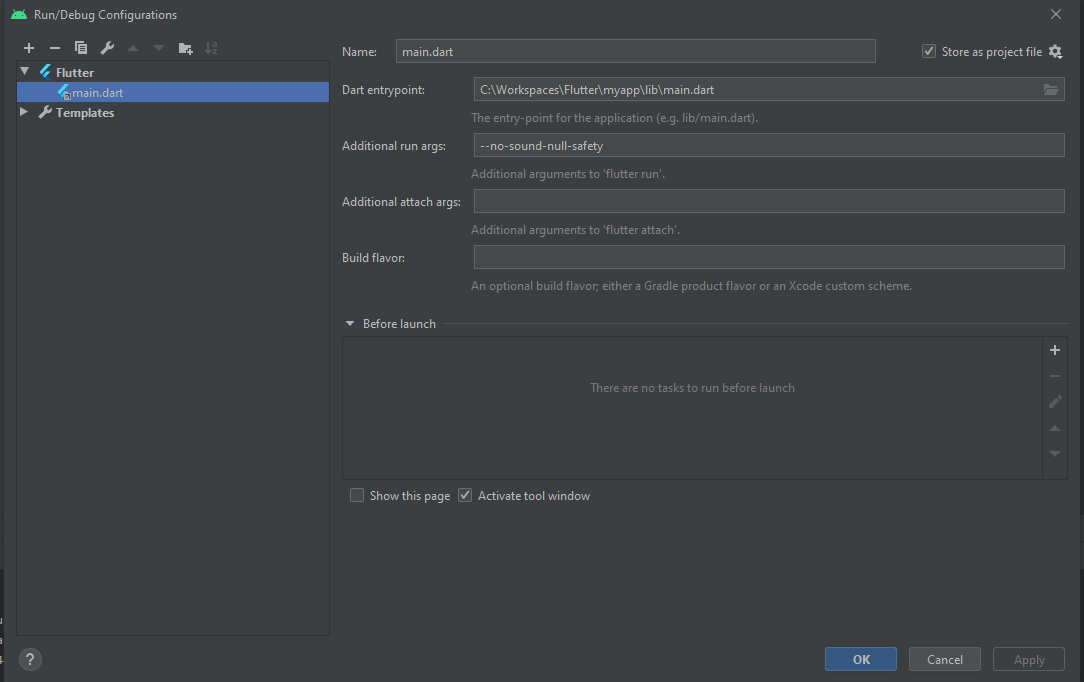
\includegraphics[width=0.7\textwidth]{capitulo2/androidstudio.png}
	\caption{Corrección del error de compilación}
	\label{cap2:001}
\end{figure} 

Después de ejecutar la compilación la salida obtenida se muestra en la figura \ref{cap2:002}.

\begin{figure}[htb]
	\centering
	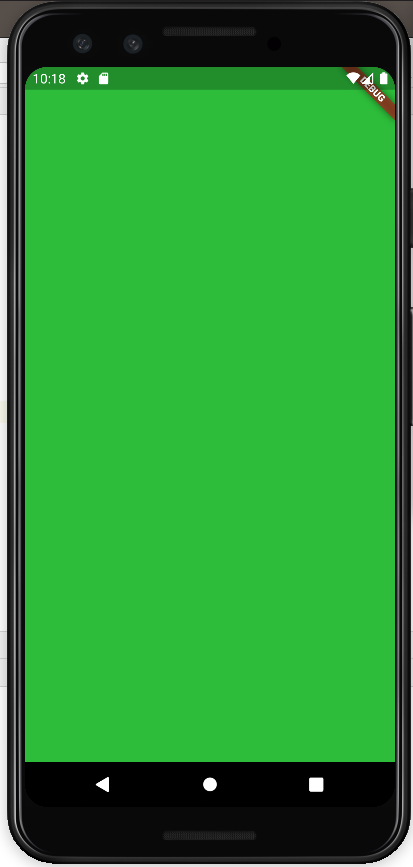
\includegraphics[width=0.4\textwidth]{capitulo2/primerPantalla.png}
	\caption{Pantalla de salida de la primera ejecución}
	\label{cap2:002}
\end{figure} 


